In this section, we will evaluate \name{}'s performance, including the localization accuracy, the performance of key sharing, and the performance of packet forwarding with \name{}.\\
%, and localization accuracy when performing fault localization.}\\
\noindent {\bf Experiment setup.} We implement \name{} protocol described in Section \ref{lakeysection}, \ref{sourceandpathverificationsection} and \ref{faultlocalization} with \namekey{} as a user-level application for carrying out secret key distribution, source and path verification, and fault localization. The prototype of the router, called \name{} router, is implemented by using Click Modular Router \cite{kohler2000click}, which runs on Ubuntu Linux 12.04 with Intel(R) Core(TM) i5-4590, CPU @ 3.30 GHz, 16GB memory and NIC of 1000 Mbps\footnote{Of course, it is also feasible for the similar packet processing as \name{} to be implemented along fast TCAM path or in commercial router \cite{basescu2016high}.}. We achieve the communications between two computers acting as the source and the destination (Intel(R) Core(TM) i5-4200U, CPU @ 1.6GHz/2.3 GHz, 12.0 GB memory) through \name{} router. In this evaluation, we use SHA-3 algorithm to compute the hash values of long strings, such as the calculation of PacketID (see Eq. \ref{packetid}). For computing the PRF value, we use HMAC based on SHA-1. We respectively truncate the value of SHA-3 and HMAC to meet our requirements, such as from 256 bits to 128 bits for computing PacketID and from 160 bits to 32 bits for computing \emph{M}$_\emph{i}$. In \namekey{}, RSA algorithm is employed to compute the signature, asymmetric encryption, and decryption. To evaluate the effect of fault localization, such as localization accuracy, we implement a multi-hop simulation network using NS3, where the source communicates the detestation through more than one intermediate routing node.
\begin{figure*}[htbp]
\centering
\subfigure[The positive ratio of different router locations for different misbehaved packet loss probabilities.]{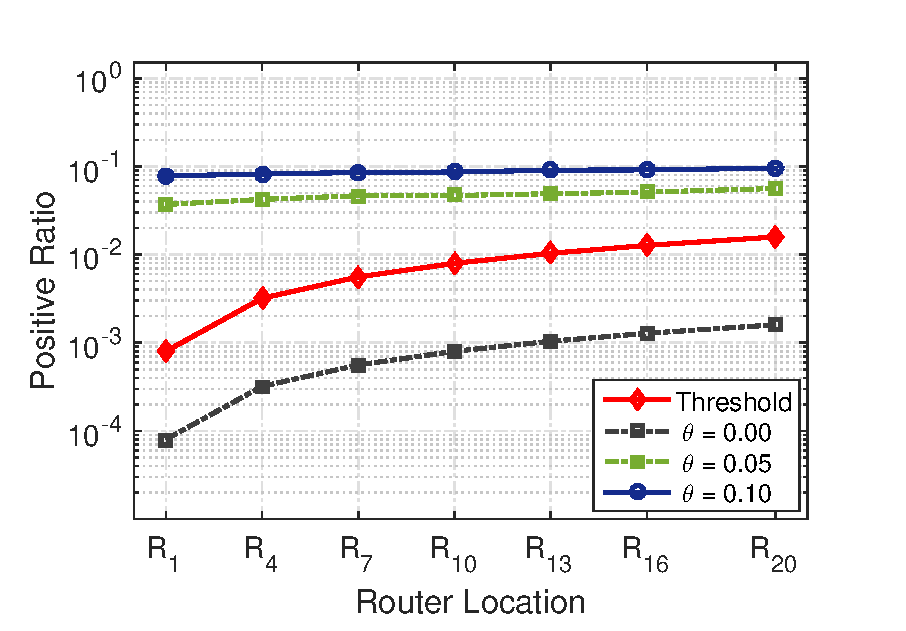
\includegraphics[width=2.3in, angle=0]{code_matlab/positiveratio11.eps}}\label{positiveratio}
\subfigure[The relationship between positive ratio and $~~~~$ $~~~~$ different packet natural loss probabilities.]{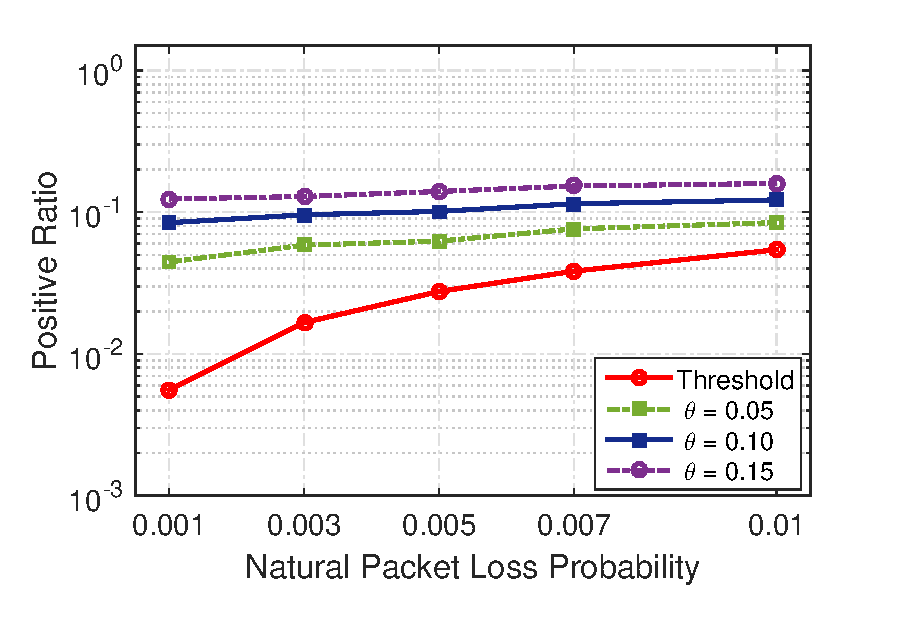
\includegraphics[width=2.3in, angle=0]{code_matlab/positiveratio22.eps}}\label{positiveratio2}
\subfigure[The localization accuracy for different packet $~~$ $~~~~$ mis-loss or natural loss probabilities.]{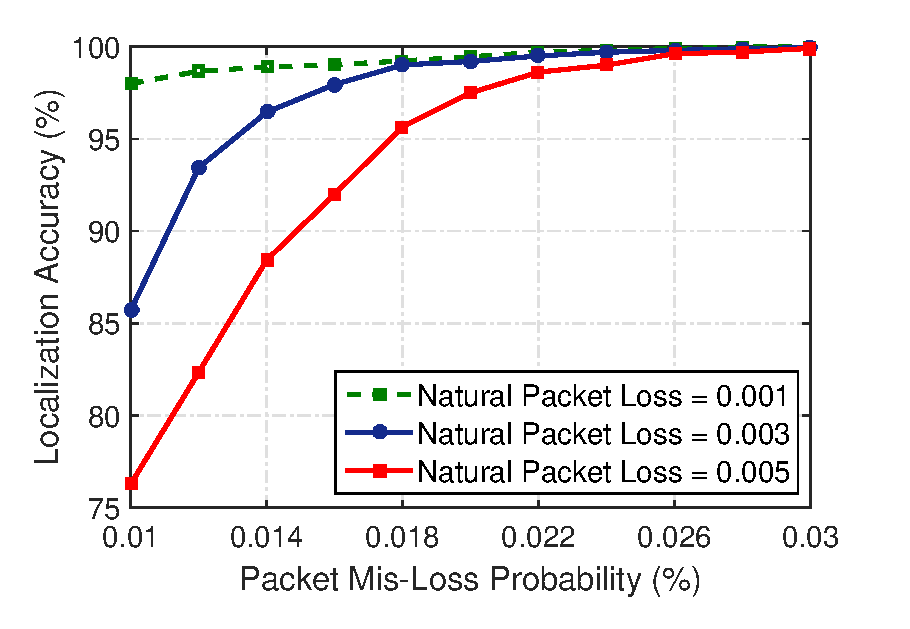
\includegraphics[width=2.3in, angle=0]{code_matlab/localizationaccuracy.eps}}\label{localizationaccuracyfig1}
\subfigure[The relationship between localization accuracy $~~~~$ and natural packet loss probability.]{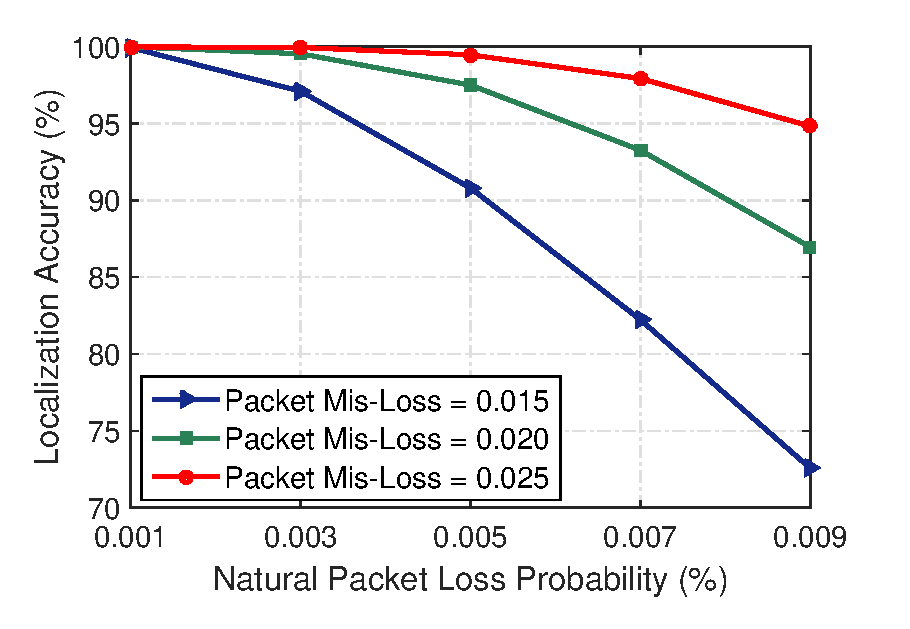
\includegraphics[width=2.3in, angle=0]{code_matlab/localizationaccuracy2.eps}}\label{localizationaccuracyfig2}
\subfigure[\name{} router's forwarding efficiency for different packet sizes under the Internet average path length.]{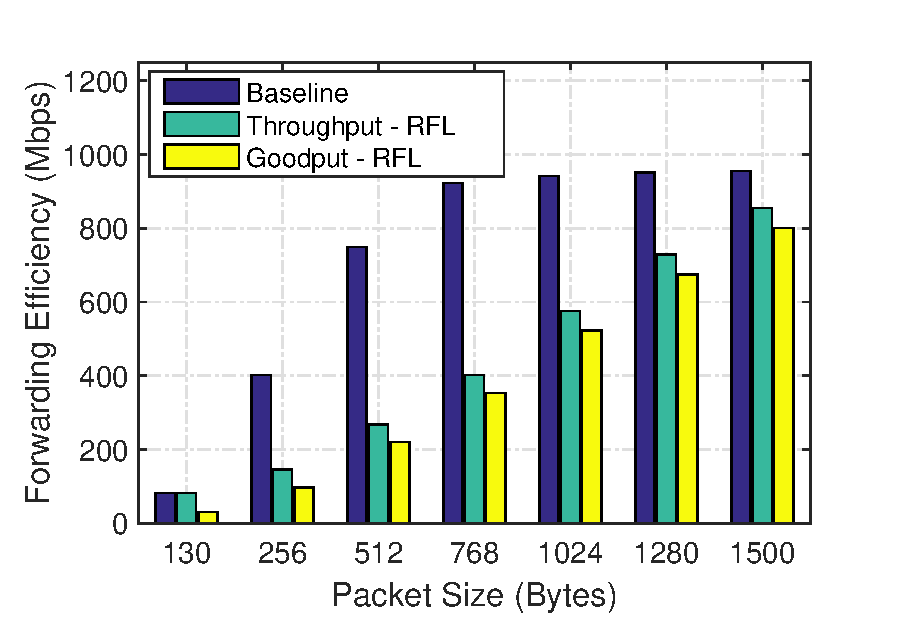
\includegraphics[width=2.3in, angle=0]{code_matlab/throughput2_spmoni.eps}}\label{packetsizeforwarding}
\subfigure[\name{} router's forwarding efficiency under different path lengths for the packet size of 1500 bytes.]{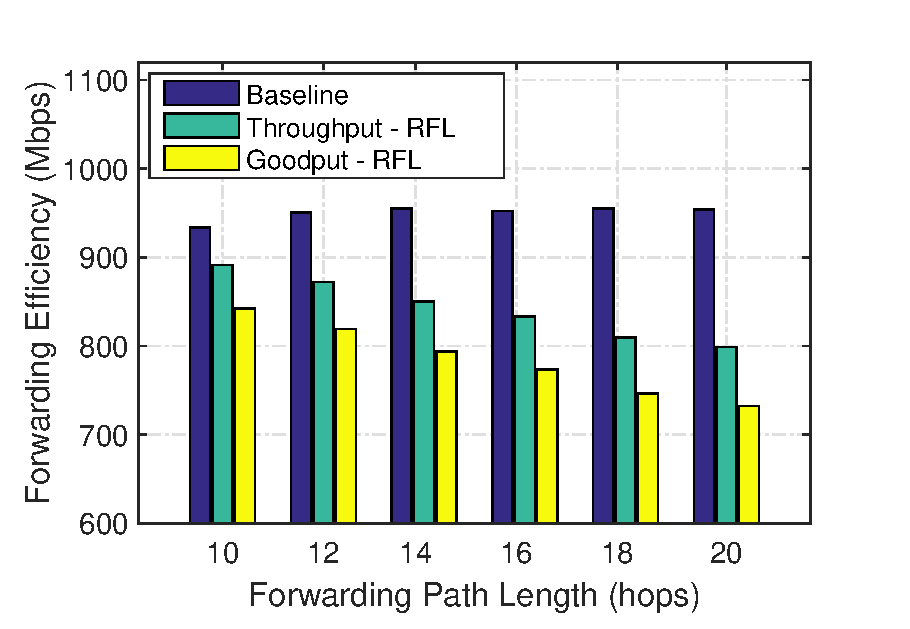
\includegraphics[width=2.3in, angle=0]{code_matlab/throughput_pathlength_spmoni2.eps}}\label{pathlengthforwarding}
\caption{The \name{} performance evaluation in terms of positive ratio, localization accuracy of fault localization, and \name{} router's forwarding efficiency.}\label{rflevaluation}
\end{figure*}
\vspace{-0.1in}
\subsection{Positive Ratio threshold}
\label{positiveratiothreshold}
%We define \emph{\textbf{positive ratio}} denoted by $\mathcal{P}_\emph{i}$ and $\mathcal{P}_\emph{D}$ for \emph{R}$_\emph{i}$ and {\tt D}, which illustrates the probability that the corresponding entity is misbehaved. When $\mathcal{P}_\emph{i}$ is larger than \emph{\textbf{positive ratio threshold}} (denoted by $\zeta$), and $\mathcal{P}_\emph{1}$, $\cdots$, $\mathcal{P}_{\emph{i-}1}$ are all less than $\zeta$, we can identify \emph{R}$_\tau$ or \emph{R}$_{\emph{i-}1}$ as the misbehaved entity (detailed in Section \ref{faultlocalization}).
We evaluate positive ratio threshold $\zeta_\emph{i}$ of $\emph{R}_\emph{i}$ through the simulation network with the path length of 20 hops, the longest forwarding path in end-to-end communication according to a CAIDA research \cite{huffaker2002distance}. The ratio illustrates the probability that the corresponding entity is misbehaved. When $\mathcal{P}_\emph{i}$ is larger than $\zeta_\emph{i}$, and $\mathcal{P}_\emph{1}$, $\cdots$, $\mathcal{P}_{\emph{i-}1}$ are respectively less than $\zeta_\emph{1}$, $\cdots$, $\zeta_{\emph{i-}1}$, we can identify \emph{R}$_\emph{i}$ or \emph{R}$_{\emph{i-}1}$ as the misbehaved entity (detailed in Section \ref{faultlocalization}). In \name{}, the attacks (including source spoofing, path hijacking, frame, and collusion attack) all lead to downstream entities' dropping the packet. %We respectively define $\theta$, $\theta_{\emph{na}}$ and $\theta_{\emph{mis}}$ as the probability of packet loss, natural loss and malicious loss (mis-loss) of the entity (including its upstream neighbored link).\\
\iffalse
\begin{figure}%[H]
  % Requires \usepackage{graphicx}
  \centering
  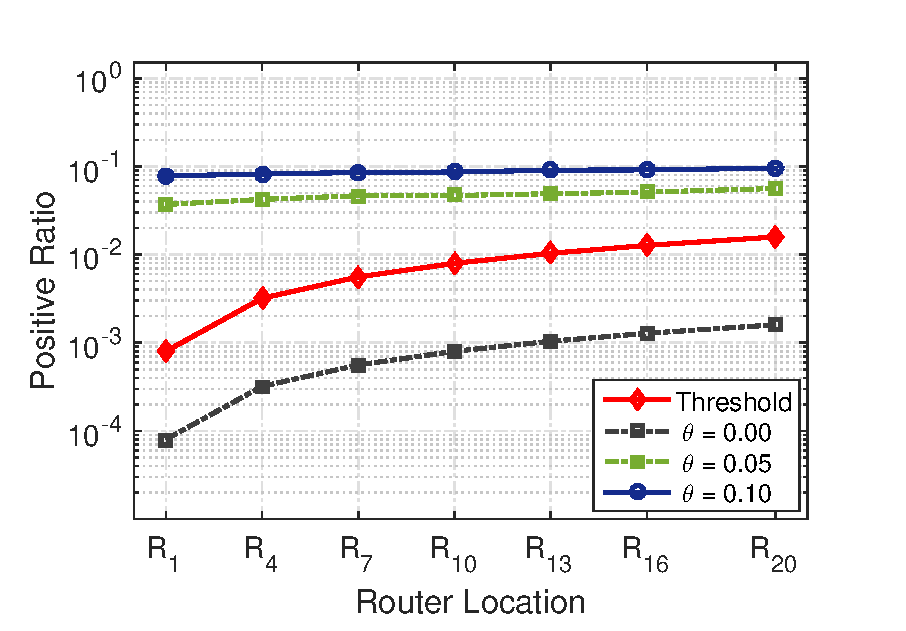
\includegraphics[width=0.85\columnwidth]{code_matlab/positiveratio11.eps}\\
  \caption{The relationship between router location (from \emph{R}$_1$ to \emph{R}$_\emph{20}$) and positive ratio with the variation of misbehaved packet loss probability.}\label{positiveratio}
\end{figure}
\begin{figure}%[H]
  % Requires \usepackage{graphicx}
  \centering
  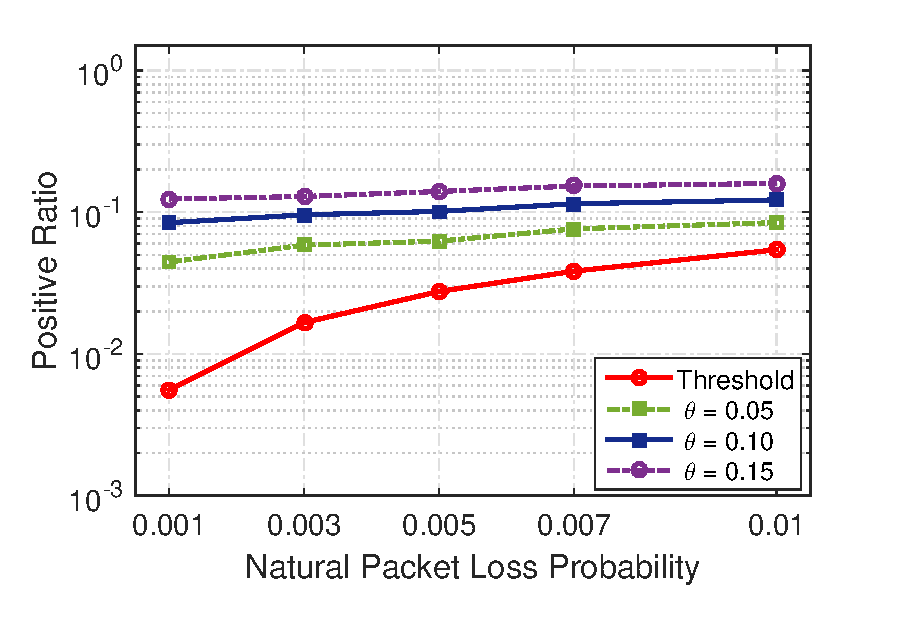
\includegraphics[width=0.85\columnwidth]{code_matlab/positiveratio22.eps}\\
  \caption{The relationship between natural packet loss probability and positive ratio with the variation of misbehaved packet loss probability.}\label{positiveratio2}
\end{figure}
\fi

Fig. \ref{rflevaluation}(a) shows the relationship between router location and its positive ratio with the variation of packet loss probability. To obtain a more accurate result, we run our simulation over 100 times for each result. The red line depicts the scenarios only with natural packet loss ($\theta_{\emph{na}}$=0.001), which is also the threshold line that helps identify the misbehaved entity. When the packet loss probability is 0.00, the positive ratio $\mathcal{P}$ is lower than the threshold value, because the lower packet loss probability brings about less packet loss during the transmission. We set one misbehaved router at different locations from \emph{R}$_1$ to \emph{R}$_{\emph{20}}$. The blue line ($\theta$=0.10) and the green dotted line ($\theta$=0.05) respectively show the positive ratio $\mathcal{P}$ of the misbehaved router in different locations. We learn that the positive $\mathcal{P_\emph{i}}$ will exceed the threshold $\zeta_\emph{i}$ when the malicious router behaves abnormally with the probability of $\theta$=0.10 or $\theta$=0.05. According to this threshold, {\tt S} can locate the misbehaved router who has different mis-loss probabilities.

We also evaluate the relationship between positive ratio and natural packet loss probabilities under different misbehaved packet loss probability. Fig. \ref{rflevaluation}(b) shows the positive ratio of the middle entity (i.e., \emph{R}$_\emph{7}$) with the average Internet forwarding path length, i.e., \emph{n}=13 hops. With the increment of natural packet loss probability, the positive ratio threshold becomes larger, because the higher loss probability introduces more packets to be dropped. When the misbehaved packet loss probability is larger than the natural loss probability, the corresponding ratios exceed the threshold value. Therefore, under different natural packet loss probabilities, the fault can also be localized in \name{} protocol.
\vspace{-0.1in}
\subsection{Fault Localization Accuracy}
\label{localizationaccuracy}
Based on the positive ratio threshold above, we evaluate the fault localization accuracy denoted by $\delta$ through a simulation scenario with 13-hop forwarding path. We set one router of random location on forwarding path as the misbehaved router, that can launch both source spoofing and path inconsistency attacks. Besides, this misbehaved router can also disturb \name{} protocol, which finally introduces the packets dropping.\\
\indent
We first evaluate the fault localization accuracy with the variation of packet mis-loss probability of misbehaved router, just as Fig. \ref{rflevaluation}(c) shows. From Fig. \ref{rflevaluation}(c), we can learn the fault localization accuracy of \name{} becomes higher with the increase of packet mis-loss probability. This is because more packet mis-loss results in higher positive ratio than the threshold, and the higher mis-loss probability make \name{} easier to identify the fault. We respectively take the value of natural packet loss probability as 0.001, 0.003 and 0.005, which introduce different positive ratio thresholds (described in Section \ref{positiveratiothreshold}). From Fig. \ref{rflevaluation}(c), we know less natural packet loss brings about higher localization accuracy, as the lower positive ratio threshold makes it easier to localize the fault. This is in line with our theoretical analysis in Section \ref{localizationaccuracyanalysis}.\\
\indent
Then the relationship between localization accuracy and natural packet loss probability is evaluated in Fig. \ref{rflevaluation}(d). With the larger range of natural packet loss, we can learn localization accuracy becomes lower when the more natural packet is dropped. Fortunately, under the smaller natural packet loss probability, such as 0.001 or 0.003, \name{} achieves the fault localization with the accuracy of over 99.5\% when the mis-loss probability is 0.020 or more.
\begin{table}
\caption{\namekey{} Evaluation - Communication Overhead}
\renewcommand\arraystretch{1.5}
\centerline{
\begin{tabular}{|p{1.8cm}<{\centering}|p{1.2cm}<{\centering}|p{1.2cm}<{\centering}|p{1.2cm}<{\centering}|}
%\toprule[2pt]
\hline
\hline
%\cline{1-1}
\centering
~&\textbf{\namekey{}} & \textbf{DRKey} & \textbf{ICING} \\\hline \hline
Source ({\tt S}) & 2 & 2 & 4$\ast$\emph{n}+4          \\\hline
Router (\emph{R}$_\emph{i}$) & 2 & 2 & 4$\ast$\emph{n}+4          \\\hline
Destination ({\tt D}) & 2 & 2 & 4$\ast$\emph{n}+4          \\\hline
%\bottomrule[2pt]
\hline
\end{tabular}
}
\begin{tablenotes}
  \item[1] Here, the communication overhead is evaluated by the number of extra packets during symmetric key distribution.
\end{tablenotes}
\label{communicationoverhead}
\end{table}
\vspace{-0.1in}
\subsection{Router Throughput and Goodput}
\label{routerthroughput}
We implement the prototype of \name{} router to evaluate the forwarding efficiency, including throughput and goodput, which can be used to demonstrate the technical feasibility in real experiments.
In order to evaluate the packet forwarding efficiency at routing entities, we use iperf \cite{tirumala2005iperf} to achieve the communications between the source and the destination through \name{} router. \name{} router performs the following operations when delivering packets: source and path validation, probabilistic packet sampling and storing sampling information. \\
\indent
From Eq. \ref{mid}, we learn the computation overhead of \name{} router increases linearly from \emph{R}$_\emph{n}$ to \emph{R}$_\emph{1}$ when recomputing the markings. Namely, \name{} routers close to {\tt S} have higher computation overhead than the router close to {\tt D} as the longer input. In this case, we evaluate the performance of middle router \emph{R}$_{[\frac{\emph{n}}{2}]}$ for the average-case analysis with different path lengths and packet sizes. Fig. \ref{rflevaluation}(e) shows the relationship between packet size and forwarding efficiency with the average Internet path length of 13 hops. We calculate goodput as the valid throughput of useful packet data, excluding \name{} header. Note that the smallest packet size is 130 bytes, including 90-byte \name{} header and 40-byte IP/TCP header. We adjust packet size of 130 bytes to 1500 bytes by configuring the interface Maximum Transmission Unit (MTU) sizes. From Fig. \ref{rflevaluation}(e), we can know both throughput and goodput of \name{} router increase with the improvement of packet size. Especially for the large packet of 1500 bytes, \name{} router can achieve over 90\% throughput and about 85\% goodput of baseline. From \cite{huffaker2002distance}, we learn that the path length of end-to-end communication is 15.3 $\pm$ 4.2 hops for IPv4 packets. Thus, we evaluate the packet forwarding efficiency with the path length of 10 hops to 20 hops in Fig. \ref{rflevaluation}(f). We can learn that \name{} router's throughput and goodput all decrease when the forwarding path length increases because more downstream routers' markings are added as the input of marking recomputation. The longer input of marking recomputation incurs lower forwarding efficiency. Concretely, with path length increment of 1 hop, the throughput and goodput will reduce by 9.26 Mbps. Fortunately, the throughput and goodput respectively exceed 850 Mbps and 800 Mbps in the networks of 13-hop path length, more than 90\% and 85\% compared to the baseline. Thus \name{} incurs only 10\% forwarding efficiency while guaranteeing the robustness of fault localization, which is an incomparable advantage of other packet verification mechanism.
\begin{table}
\caption{\namekey{} Evaluation - ReqKey and AckKey Packet Latency}
\renewcommand\arraystretch{1.5}%{\multirowsetup}{\centering}
\centerline{
\begin{tabular}{|p{1.6cm}<{\centering}|p{1.8cm}<{\centering}|p{1.7cm}<{\centering}|p{1.7cm}<{\centering}|} %|r|c|l|}%\multirow{5}{2cm}{Source}
%\toprule[2pt]
\hline
\hline
%\cline{1-1}
\centering
&\textbf{Entity} & \textbf{Path Length} & \textbf{Latency} \\\hline \hline
& Source ({\tt S})  & Irrelevant           & 653 $\mu$s           \\\cline{2-4}
ReqKey & Router (\emph{R}$_\emph{i}$) & Irrelevant          & 548 $\mu$s           \\\cline{2-4}
& Destination ({\tt D})  & Irrelevant          & 627 $\mu$s           \\\hline \hline
& & 11           &  13128 $\mu$s           \\\cline{3-4}
& & 13           &  16534 $\mu$s           \\\cline{3-4}
& Source ({\tt S}) & 15           &  20176 $\mu$s           \\\cline{3-4}
AckKey &                 & 17           &  24051 $\mu$s           \\\cline{3-4}
&                 & 19           &  28815 $\mu$s           \\\cline{2-4}
& Router (\emph{R}$_\emph{i}$)  & Irrelevant          & 903 $\mu$s           \\\cline{2-4}
& Destination ({\tt D})         & Irrelevant          & 754 $\mu$s           \\\cline{2-4} \hline\hline
%\bottomrule[2pt]
\end{tabular}
}
\label{ackkeypacketlatencytable}
\end{table}
\vspace{-0.1in}
\subsection{Performance and Overhead of \namekey{}}
\label{laskeyevaluation}
To demonstrate the feasibility of \namekey{} in the early stage of \name{} protocol, we perform \namekey{} performance evaluation during symmetric key distribution. The evaluation results show that \namekey{} introduces the low communication overhead and packet latency. %The storage overhead has been analyzed in Section \ref{storageoverhead}.

Table \ref{communicationoverhead} provides the results of communication overhead (evaluated by the number of extra packets) at the source ({\tt S}), the router (\emph{R}$_\emph{i}$) and the destination ({\tt D}). We can learn \namekey{} achieves the same lower communication overhead with the state-of-the-art scheme DRKey \cite{kim2014lightweight}, and outperforms than ICING \cite{naous2011verifying}. Note that \namekey{} and DRKey all require only 2 additional packets as the communication overhead for the symmetric key establishment, while ICING needs 4$\ast$\emph{n}+4 extra packets on all entities.

More importantly, \namekey{} achieves a more secure and robust symmetric key distribution than the state-of-the-art scheme DRKey. On one hand, if any misbehaved router disturbs secret key distribution by means of dropping, modifying or redirecting \emph{request} or \emph{ack} packet, DRKey scheme will fail. However, \namekey{} enables each entity to verify the \emph{request} or \emph{ack} message. If any failure occurs or the timer expires, the entity will send its encrypted symmetric key back to {\tt S}. In this case, {\tt S} can still obtain reliable entities' symmetric key even if there is any router trying to disturb secret key establishment. On the other hand, if any misbehaved router disturbs key distribution, DRKey will be stranded, resulting in {\tt S}'s wasting time to wait for ack message. However, \namekey{} can realize it as soon as possible with the help of timer, and localize the fault who disturbs secret key distribution. In this case, {\tt S} can adjust the policies (e.g., avoiding the localized misbehaved router or correcting the fault) based on the result of fault localization.
\iffalse
\begin{table}
\caption{\namekey{} Evaluation - ReqKey Packet Latency}
\renewcommand\arraystretch{1.5}
\centerline{
\begin{tabular}{|p{2cm}<{\centering}|p{2cm}<{\centering}|p{2cm}<{\centering}|p{2cm}<{\centering}|}
%\toprule[2pt]
\hline
\hline
%\cline{1-1}
\centering
\textbf{Entity} & \textbf{Path Length} & \textbf{Latency} \\\hline \hline
Source ({\tt S})  & Irrelevant           & 653 $\mu$s           \\\hline
Router (\emph{R}$_\emph{i}$) & Irrelevant          & 548 $\mu$s           \\\hline
Destination ({\tt D})  & Irrelevant          & 627 $\mu$s           \\\hline
%\bottomrule[2pt]
\hline
\end{tabular}
}
\label{reqkeypacketlatency}
\end{table}
\fi

To evaluate packet latency during \namekey{} processing, we implement the prototype of \namekey{} on the source host, the RFL router, and the destination host. \namekey{} scheme contains two stages: ReqKey stage and AckKey stage. From Section \ref{reqkeytransmission}, we can learn the packet latency on different entities is irrelevant to path length on ReqKey stage. In this case, we will ignore the effect of path length changes on entities' performance. \\
\indent Table \ref{ackkeypacketlatencytable} shows the packet latency of ReqKey stage and AckKey stage on the source, intermediate routers, and the destination. We can learn the packet latency of \namekey{} on the source is affected by path length, especially on AckKey stage. That is mainly because the source will check all the signatures and decrypts the encrypted symmetric keys when receiving AckKey packet, leading to higher computation overhead in proportion to path length. This result also shows the packet latency on RFL router is smaller than at least one of end hosts, which enables more cycles to be used to distribute secret keys by the source or the destination. 
\iffalse
\begin{figure}%[H]
  % Requires \usepackage{graphicx}
  \centering
  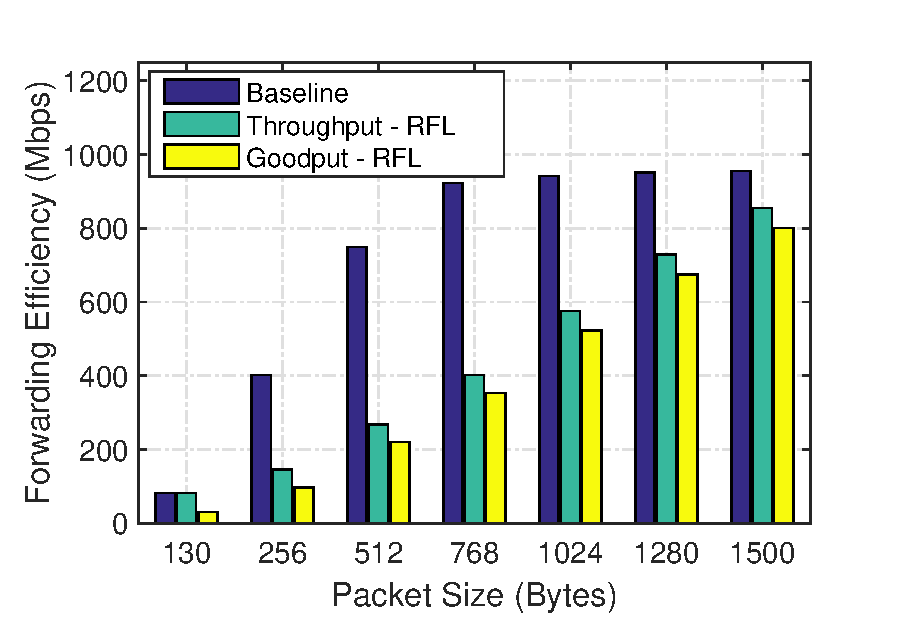
\includegraphics[width=6cm]{code_matlab/throughput2_spmoni.eps}\\
  \caption{\name{} router's forwarding efficiency (throughput and goodput) for IPv4 packets of 130 bytes to 1500 bytes, with the path length of 13 hops.}\label{packetsize}
\end{figure}
\begin{figure}%[H]
  % Requires \usepackage{graphicx}
  \centering
  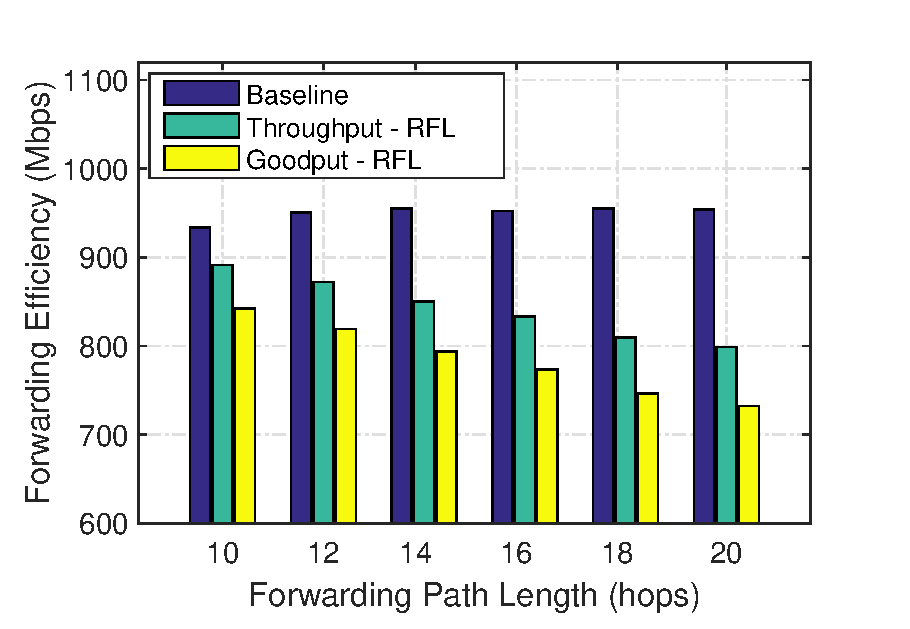
\includegraphics[width=6cm]{code_matlab/throughput_pathlength_spmoni2.eps}\\
  \caption{\name{} router's forwarding efficiency (throughput and goodput) for data-plane networks of 10 hops to 20 hops, with packet size of 1500 bytes.}\label{pathlength}
\end{figure}
\begin{figure}%[H]
  % Requires \usepackage{graphicx}
  \centering
  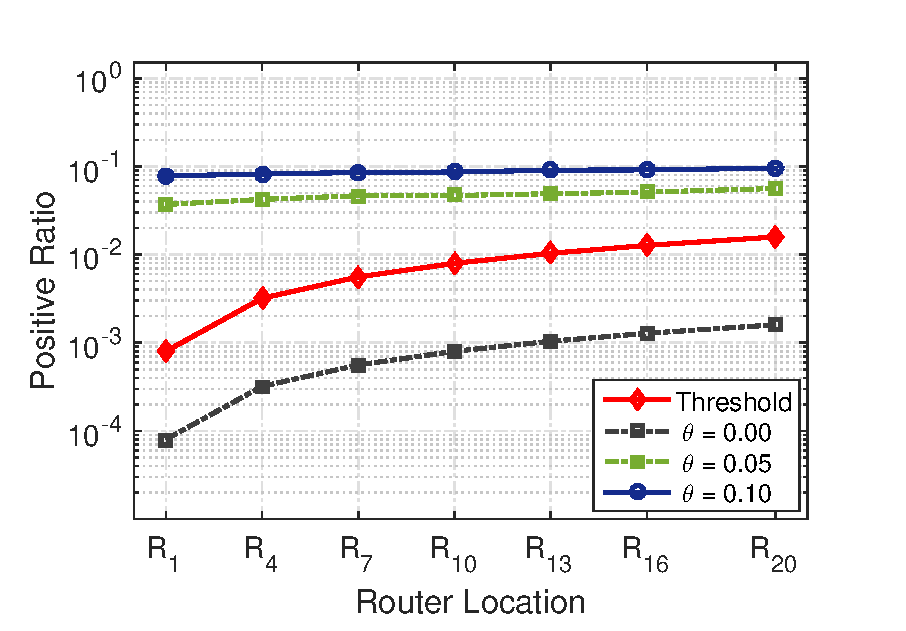
\includegraphics[width=6cm]{code_matlab/positiveratio11.eps}\\
  \caption{The relationship between router location (from \emph{R}$_1$ to \emph{R}$_\emph{20}$) and positive ratio with the variation of misbehaved packet loss probability.}\label{positiveratio}
\end{figure}
\begin{figure}%[H]
  % Requires \usepackage{graphicx}
  \centering
  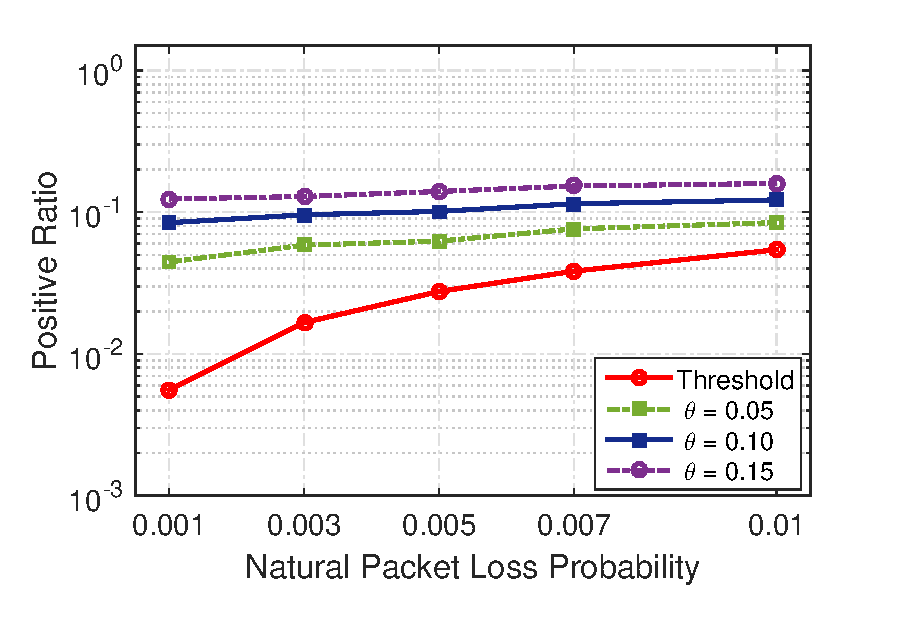
\includegraphics[width=6cm]{code_matlab/positiveratio22.eps}\\
  \caption{The relationship between natural packet loss probability and positive ratio with the variation of misbehaved packet loss probability.}\label{positiveratio2}
\end{figure}
\begin{figure}%[H]
  % Requires \usepackage{graphicx}
  \centering
  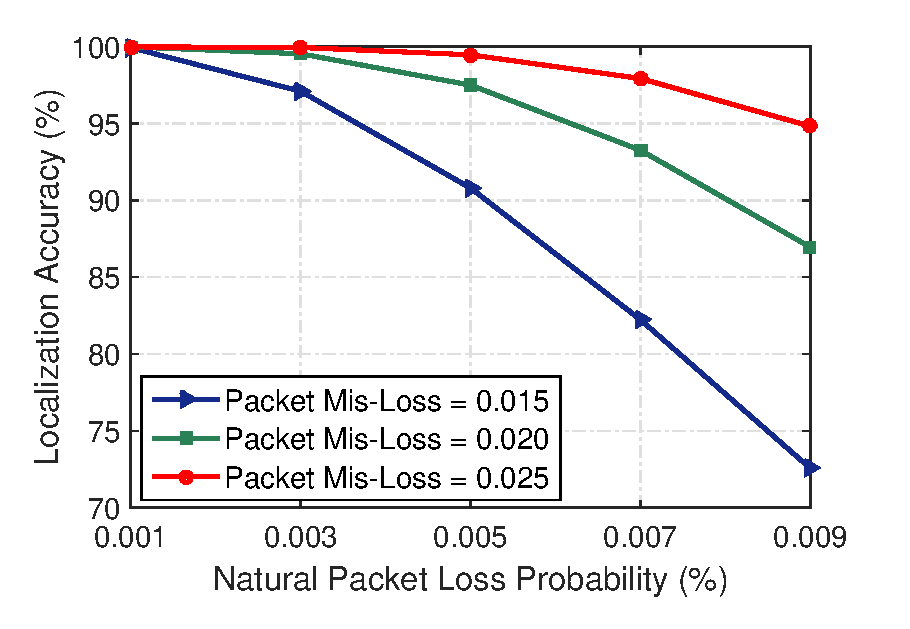
\includegraphics[width=6cm]{code_matlab/localizationaccuracy2.eps}\\
  \caption{The relationship between localization accuracy $\delta$ and natural packet loss probability with the different packet mis-loss simulation scenario.}\label{localizationaccuracyfig2}
\end{figure}
\begin{figure}%[H]
  % Requires \usepackage{graphicx}
  \centering
  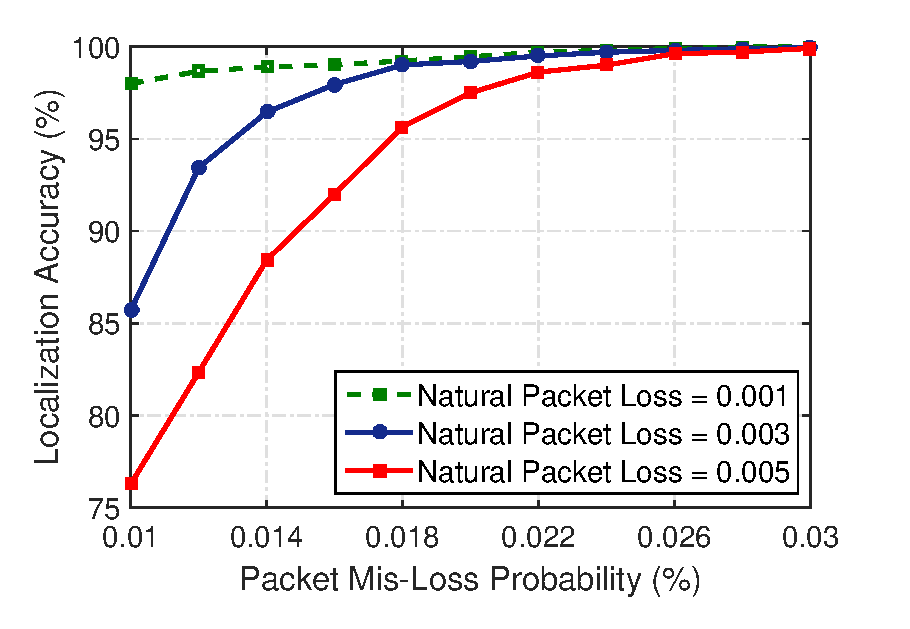
\includegraphics[width=6cm]{code_matlab/localizationaccuracy.eps}\\
  \caption{The relationship between localization accuracy $\delta$ and packet mis-loss probability with different natural packet loss in simulation scenario.}\label{localizationaccuracyfig1}
\end{figure}
\fi
%\vspace{-0.1in}
